\documentclass[11pt, a4paper]{article}
\usepackage[utf8]{inputenc}
\usepackage[T1]{fontenc}
\usepackage[english]{babel}
\usepackage{geometry}
\usepackage{booktabs}
\usepackage{hyperref}
\usepackage{lmodern}
\usepackage{graphicx}
\usepackage{amssymb} % For checkmark and math symbols
\usepackage[table]{xcolor} % Ajout pour la couleur des tableaux
\usepackage{pgfplots} % Ajout pour les graphiques
\usepackage{soul} % For text highlighting
\pgfplotsset{compat=1.18} % Spécifier une version de compatibilité

% Couleurs personnalisées (consistent severity palette)
\definecolor{lightgreen}{rgb}{0.85,1,0.85}
\definecolor{lightorange}{rgb}{1,0.9,0.8}
\definecolor{lightred}{rgb}{1,0.8,0.8}
\definecolor{vuln-critical}{rgb}{0.8,0.1,0.1}  % Dark red
\definecolor{vuln-high}{rgb}{1,0.4,0}          % Orange
\definecolor{vuln-medium}{rgb}{1,0.8,0}        % Yellow
\definecolor{vuln-low}{rgb}{0.4,0.6,0.9}       % Light blue
\definecolor{gantt-supported}{rgb}{0.2,0.7,0.3}
\definecolor{gantt-eol}{rgb}{0.8,0.2,0.2}
\definecolor{highlight}{rgb}{1,1,0.7}          % Light yellow for highlighting


% Configuration des marges
\geometry{a4paper, margin=1in}

% Configuration des liens hypertextes
\hypersetup{
    colorlinks=true,
    linkcolor=blue,
    urlcolor=blue,
    pdftitle={PostgreSQL Security Analysis},
    pdfauthor={Adrien SALES (@rastadidi)},
    pdfsubject={Security, PostgreSQL, Vulnerabilities, DevOps},
    pdfkeywords={PostgreSQL, security, vulnerability, DevOps, DevSecOps, SecOPS, docker, trivy, geol}
}

% Titre et auteur
\title{PostgreSQL Security Analysis\\ \large with \texttt{geol} and \texttt{trivy} tools \\ github.com/adriens/geol-showcase}
\author{Gemini CLI | \texttt{geol} | \texttt{trivy} | Adrien SALES ($\mathbf{X}$ \texttt{@rastadidi})}
\date{\today}

\begin{document}

\maketitle

\begin{abstract}
This article presents a concise analysis of the security and lifecycle of
the \href{https://www.postgresql.org/}{PostgreSQL} database versions.

Using the \href{https://github.com/opt-nc/geol}{\texttt{geol}} tool to check End-of-Life dates and \href{https://trivy.dev/}{\texttt{trivy}} to scan vulnerabilities in official Docker images, I establish a risk profile for currently supported and unsupported versions.\\

The goal is to demonstrate the crucial importance of using maintained versions and the value of combining generative AI with optimally designed CLI tools to automate and enrich this type of analysis.
\end{abstract}

\tableofcontents
\newpage

\section{Executive Summary}

\textbf{Key Findings:}

\begin{itemize}
    \item \textbf{\textcolor{gantt-supported}{5 Supported Versions:}} PostgreSQL versions 14-18 are actively maintained with EOL dates ranging from 2026 to 2030.
    \item \textbf{\textcolor{gantt-eol}{Fresh EOL Alert:}} PostgreSQL 13 recently reached end-of-life on November 13, 2025, joining versions 9.6-12 as unsupported.
    \item \textbf{\textcolor{vuln-critical}{Security Gap:}} Unsupported versions contain \textbf{\textcolor{vuln-critical}{2-10× more vulnerabilities}} than supported versions, with critical CVEs present only in EOL versions.
    \item \textbf{Patch Impact:} Minor updates are crucial - PostgreSQL 18.1 reduced vulnerabilities by \textbf{\textcolor{gantt-supported}{22\%}} compared to 18.0 (204 → 159 total vulnerabilities).
    \item \textbf{\textcolor{vuln-critical}{Critical Recommendation:}} Migrate immediately from any version $\leq$13 to version $\geq$14. The security risk of unsupported versions is unacceptable for production environments.
\end{itemize}

\textbf{Risk Profile Summary:}
\begin{itemize}
    \item $\checkmark$ \textbf{\textcolor{gantt-supported}{Low Risk:}} Versions 14-18 (0-1 critical, 6-17 high vulnerabilities)
    \item $\times$ \textbf{\textcolor{gantt-eol}{High Risk:}} Versions 9.6-13 (7-10 critical, 70-97 high vulnerabilities)
\end{itemize}

\section{Introduction to the Tools}

Maintaining a secure software infrastructure relies on two fundamental pillars:

\begin{itemize}
    \item \textbf{Actively supported versions}
    \item \textbf{Awareness of vulnerabilities} present in the components we deploy
\end{itemize}

Below is a quick overview of the tools used for this analysis.

\subsection{\texttt{geol}: The Lifecycle Guardian}

\href{https://github.com/opt-nc/geol}{\texttt{geol}} (version 2.7.1) is a tool that queries the \href{https://endoflife.date}{endoflife.date} API to instantly retrieve software End-of-Life dates.

\subsection{\texttt{trivy}: The Vulnerability Scanner}
\href{https://trivy.dev/}{\texttt{trivy}} (version 0.69.1) is an open-source scanner that detects vulnerabilities (CVEs) in container images, file systems, and Git repositories. The vulnerability database is version 2.

\subsection{\texttt{gemini-cli}: AI Assistant}
\href{https://github.com/google-gemini/gemini-cli}{\texttt{gemini-cli}} (version 0.28.2) is an open-source AI agent that brings Gemini's power directly to the terminal.

\subsection{\LaTeX{}: Report Generator}

\LaTeX{} is a document composition system that produces high-quality technical and scientific reports. We use \texttt{xelatex} for compilation. It is particularly suited for structuring, formatting, and presenting security analysis results clearly and professionally.

\section{PostgreSQL Overview}

PostgreSQL \href{https://www.postgresql.org/}{https://www.postgresql.org/}, also known as Postgres, is a free and open-source relational database management system (RDBMS) emphasizing extensibility and technical standards compliance.

Postgres recommends that all users run the latest available minor release for whatever major version is in use.

The PostgreSQL Global Development Group supports a major version for 5 years after its initial release. After its five-year anniversary, a major version will have one last minor release containing any fixes and will be considered end-of-life (EOL) and no longer supported.

The Release roadmap \href{https://www.postgresql.org/developer/roadmap/}{https://www.postgresql.org/developer/roadmap/} lists upcoming minor and major releases. If the release team determines that a critical bug or security fix is too important to wait until the regularly scheduled minor release, it may make a release available outside the minor release roadmap.

A Feature Matrix \href{https://www.postgresql.org/about/featurematrix/}{https://www.postgresql.org/about/featurematrix/} documents feature availability against major releases.

\section{Methodology}

The analysis for this report was conducted on \today. The data was gathered using the following open-source tools and commands:

\begin{itemize}
    \item \textbf{Lifecycle Data:} PostgreSQL version lifecycle information was retrieved using the \texttt{geol} CLI with the command:
    \begin{verbatim}
        geol product extended psql -n0
    \end{verbatim}
    \item \textbf{Vulnerability Scanning:} Docker images for each major PostgreSQL version were scanned for vulnerabilities using the \texttt{trivy} CLI. An example command for a single version is:
    \begin{verbatim}
        trivy image postgres:18
    \end{verbatim}
\end{itemize}

\newpage

\section{Data Analysis}

\subsection{Version Lifecycle (\texttt{geol} data)}

The first step is to determine which versions are officially supported.\\

An unsupported version is a \textbf{gateway to unpatched vulnerabilities.}

\begin{table}[htbp]
\centering
\caption{PostgreSQL Version Lifecycle}
\label{tab:geol}
\begin{tabular}{@{}lccccl@{}}
	
	\textbf{Version} & \textbf{Release Date} & \textbf{Latest} & \textbf{Latest Release} & \textbf{End of Support (EOL)} & \textbf{Status} \\ \midrule
\rowcolor{lightgreen} 18 & 2025-09-25 & 18.2 & 2026-02-09 & 2030-11-14 & $\checkmark$ Supported \\
\rowcolor{lightgreen} 17 & 2024-09-26 & 17.7 & 2025-11-10 & 2029-11-08 & $\checkmark$ Supported \\
\rowcolor{lightgreen} 16 & 2023-09-14 & 16.11 & 2025-11-10 & 2028-11-09 & $\checkmark$ Supported \\
\rowcolor{lightgreen} 15 & 2022-10-13 & 15.15 & 2025-11-10 & 2027-11-11 & $\checkmark$ Supported \\
\rowcolor{lightgreen} 14 & 2021-09-30 & 14.20 & 2025-11-10 & 2026-11-12 & $\checkmark$ Supported \\
\rowcolor{lightred} 13 & 2020-09-24 & 13.23 & 2025-11-10 & 2025-11-13 & $\times$ \textbf{Unsupported} \\ \midrule
\rowcolor{lightred} 12 & 2019-10-03 & 12.22 & 2024-11-18 & 2024-11-21 & $\times$ \textbf{Unsupported} \\
\rowcolor{lightred} 11 & 2018-10-18 & 11.22 & 2023-11-06 & 2023-11-09 & $\times$ \textbf{Unsupported} \\
\rowcolor{lightred} 10 & 2017-10-05 & 10.23 & 2022-11-07 & 2022-11-10 & $\times$ \textbf{Unsupported} \\
\rowcolor{lightred} 9.6 & 2016-09-29 & 9.6.24 & 2021-11-08 & 2021-11-11 & $\times$ \textbf{Unsupported} \\ \bottomrule
\end{tabular}
\end{table}


\subsection{Vulnerability Analysis (\texttt{trivy} data)}

The second step is to analyze the "attack surface" of Docker images. It's important to note that while we use major version Docker tags (e.g., \texttt{postgres:18}), these tags typically point to the latest patch release within that major version series (e.g., \texttt{postgres:18} currently refers to \texttt{postgres:18.1}).

Table \ref{tab:trivy} and Figure \ref{fig:vuln-chart} show the results.

\begin{table}[htbp]
\centering
\caption{Vulnerability Summary by Version}
\label{tab:trivy}
\begin{tabular}{@{}lccccc@{}}
	\textbf{Docker Tag} & \textbf{Critical} & \textbf{High} & \textbf{Medium} & \textbf{Low} & \textbf{Total} \\ \midrule
\rowcolor{lightgreen} \texttt{postgres:18.2} & 1 & 17 & 39 & 102 & 159 \\
\rowcolor{lightgreen} \texttt{postgres:17} & 0 & 6 & 9 & 98 & 117 \\
\rowcolor{lightgreen} \texttt{postgres:16} & 0 & 6 & 9 & 98 & 113 \\
\rowcolor{lightgreen} \texttt{postgres:15} & 0 & 6 & 9 & 98 & 113 \\
\rowcolor{lightgreen} \texttt{postgres:14} & 0 & 6 & 9 & 98 & 113 \\
\rowcolor{lightred} \texttt{postgres:13} & 0 & 6 & 9 & 98 & 113 \\ \midrule
\rowcolor{lightred} \texttt{postgres:12} & 9 & 70 & 100 & 124 & 305 \\
\rowcolor{lightred} \texttt{postgres:11} & 7 & 84 & 52 & 49 & 192 \\
\rowcolor{lightred} \texttt{postgres:10} & 7 & 84 & 52 & 49 & 192 \\
\rowcolor{lightred} \texttt{postgres:9.6} & 10 & 97 & 57 & 49 & 213 \\ \bottomrule
\end{tabular}
\end{table}

\begin{figure}[htbp]
\centering
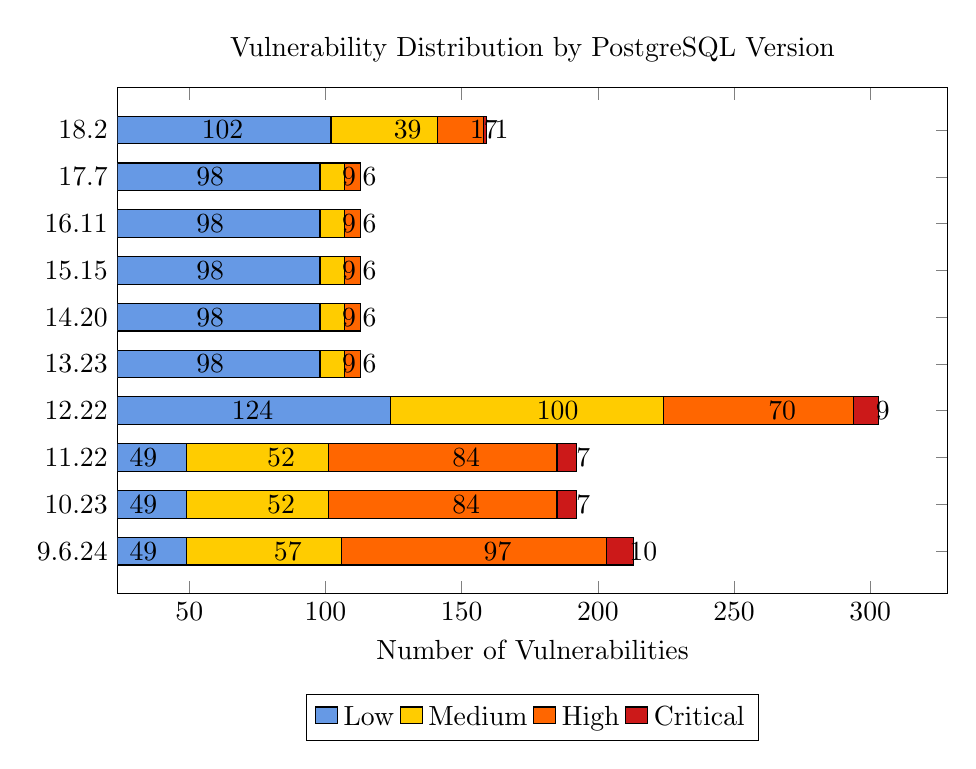
\begin{tikzpicture}
\begin{axis}[
    xbar stacked,
    width=\textwidth,
    height=8cm,
    title={Vulnerability Distribution by PostgreSQL Version},
    xlabel={Number of Vulnerabilities},
    symbolic y coords={9.6.24, 10.23, 11.22, 12.22, 13.23, 14.20, 15.15, 16.11, 17.7, 18.2},
    ytick=data,
    nodes near coords,
    nodes near coords align={horizontal},
    every node near coords/.style={
        font=\tiny,
        color=black,
        /pgf/number format/precision=0,
        /pgf/number format/fixed,
        /pgf/number format/zerofill=false
    },
    legend style={at={(0.5,-0.2)}, anchor=north, legend columns=-1}
]
\addplot[fill=vuln-low] coordinates {(102,18.2) (98,17.7) (98,16.11) (98,15.15) (98,14.20) (98,13.23) (124,12.22) (49,11.22) (49,10.23) (49,9.6.24)};
\addplot[fill=vuln-medium] coordinates {(39,18.2) (9,17.7) (9,16.11) (9,15.15) (9,14.20) (9,13.23) (100,12.22) (52,11.22) (52,10.23) (57,9.6.24)};
\addplot[fill=vuln-high] coordinates {(17,18.2) (6,17.7) (6,16.11) (6,15.15) (6,14.20) (6,13.23) (70,12.22) (84,11.22) (84,10.23) (97,9.6.24)};
\addplot[fill=vuln-critical] coordinates {(1,18.2) (0,17.7) (0,16.11) (0,15.15) (0,14.20) (0,13.23) (9,12.22) (7,11.22) (7,10.23) (10,9.6.24)};
\legend{Low, Medium, High, Critical}
\end{axis}
\end{tikzpicture}
\caption{Comparison of vulnerabilities detected by \texttt{trivy}.}
\label{fig:vuln-chart}
\end{figure}


\subsection{Critical CVE Examples}

To illustrate the concrete security risks of using unsupported versions, here are real critical vulnerabilities detected in PostgreSQL 12 (EOL November 2024):

\begin{table}[htbp]
\centering
\caption{Sample Critical CVEs in Unsupported Version (postgres:12)}
\label{tab:cve-examples}
\small
\begin{tabular}{@{}p{3cm}p{10cm}@{}}
\toprule
\textbf{CVE ID} & \textbf{Description} \\ \midrule
\href{https://nvd.nist.gov/vuln/detail/CVE-2025-15467}{CVE-2025-15467} & \textbf{OpenSSL}: Remote code execution or Denial of Service via oversized Initialization Vector in CMS parsing \\
\href{https://nvd.nist.gov/vuln/detail/CVE-2024-56171}{CVE-2024-56171} & \textbf{libxml2}: Use-After-Free vulnerability leading to potential remote code execution \\
\href{https://nvd.nist.gov/vuln/detail/CVE-2025-49794}{CVE-2025-49794} & \textbf{libxml}: Heap use-after-free (UAF) leads to Denial of Service (DoS) \\
\href{https://nvd.nist.gov/vuln/detail/CVE-2025-7458}{CVE-2025-7458} & \textbf{sqlite}: Integer overflow vulnerability enabling potential exploitation \\
\href{https://nvd.nist.gov/vuln/detail/CVE-2025-6965}{CVE-2025-6965} & \textbf{sqlite}: Integer truncation vulnerability in SQLite library \\
\bottomrule
\end{tabular}
\end{table}

\textbf{Key Takeaway:} These critical CVEs affect core dependencies (OpenSSL, libxml2, SQLite) bundled in the Docker image. Unsupported versions will never receive patches for these vulnerabilities, leaving systems permanently exposed.


\subsection{Version Lifecycle Timeline}

\begin{figure}[htbp]
\centering
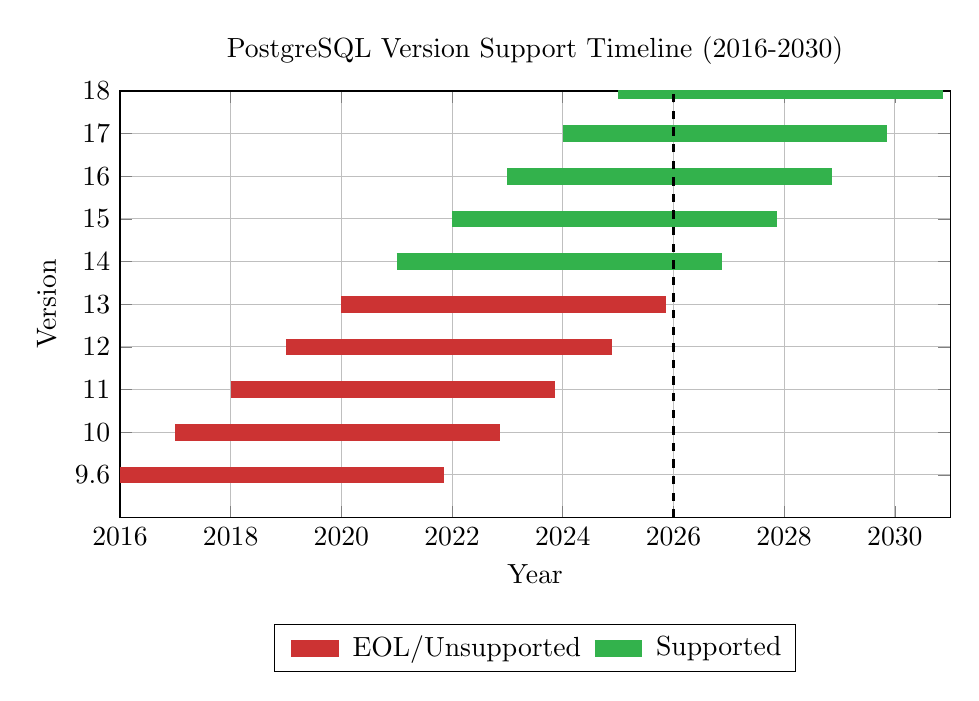
\begin{tikzpicture}
\begin{axis}[
    width=\textwidth,
    height=7cm,
    title={PostgreSQL Version Support Timeline (2016-2030)},
    xlabel={Year},
    ylabel={Version},
    xmin=2016, xmax=2031,
    ymin=0, ymax=10,
    ytick={1,2,3,4,5,6,7,8,9,10},
    yticklabels={9.6, 10, 11, 12, 13, 14, 15, 16, 17, 18},
    grid=major,
    legend style={at={(0.5,-0.25)}, anchor=north, legend columns=2},
    xticklabel style={/pgf/number format/set thousands separator={}}
]

% Unsupported versions (EOL periods)
\addplot[gantt-eol, line width=6pt] coordinates {(2016,1) (2021.86,1)}; % 9.6: 2016-2021.86
\addlegendentry{EOL/Unsupported}
\addplot[gantt-eol, line width=6pt, forget plot] coordinates {(2017,2) (2022.86,2)}; % 10: 2017-2022.86
\addplot[gantt-eol, line width=6pt, forget plot] coordinates {(2018,3) (2023.86,3)}; % 11: 2018-2023.86
\addplot[gantt-eol, line width=6pt, forget plot] coordinates {(2019,4) (2024.89,4)}; % 12: 2019-2024.89
\addplot[gantt-eol, line width=6pt, forget plot] coordinates {(2020,5) (2025.87,5)}; % 13: 2020-2025.87

% Supported versions
\addplot[gantt-supported, line width=6pt] coordinates {(2021,6) (2026.87,6)}; % 14: 2021-2026.87
\addlegendentry{Supported}
\addplot[gantt-supported, line width=6pt, forget plot] coordinates {(2022,7) (2027.87,7)}; % 15: 2022-2027.87
\addplot[gantt-supported, line width=6pt, forget plot] coordinates {(2023,8) (2028.86,8)}; % 16: 2023-2028.86
\addplot[gantt-supported, line width=6pt, forget plot] coordinates {(2024,9) (2029.86,9)}; % 17: 2024-2029.86
\addplot[gantt-supported, line width=6pt, forget plot] coordinates {(2025,10) (2030.87,10)}; % 18: 2025-2030.87

% Current date marker
\addplot[black, dashed, line width=1pt, forget plot] coordinates {(2026,0) (2026,10.5)};
\node at (axis cs:2026,10.5) [above] {\small Today};

\end{axis}
\end{tikzpicture}
\caption{PostgreSQL version support periods showing 5-year lifecycle policy. Supported versions shown in green, EOL versions in red.}
\label{fig:timeline}
\end{figure}


\subsection{Vulnerability Heat Map}

\begin{figure}[htbp]
\centering
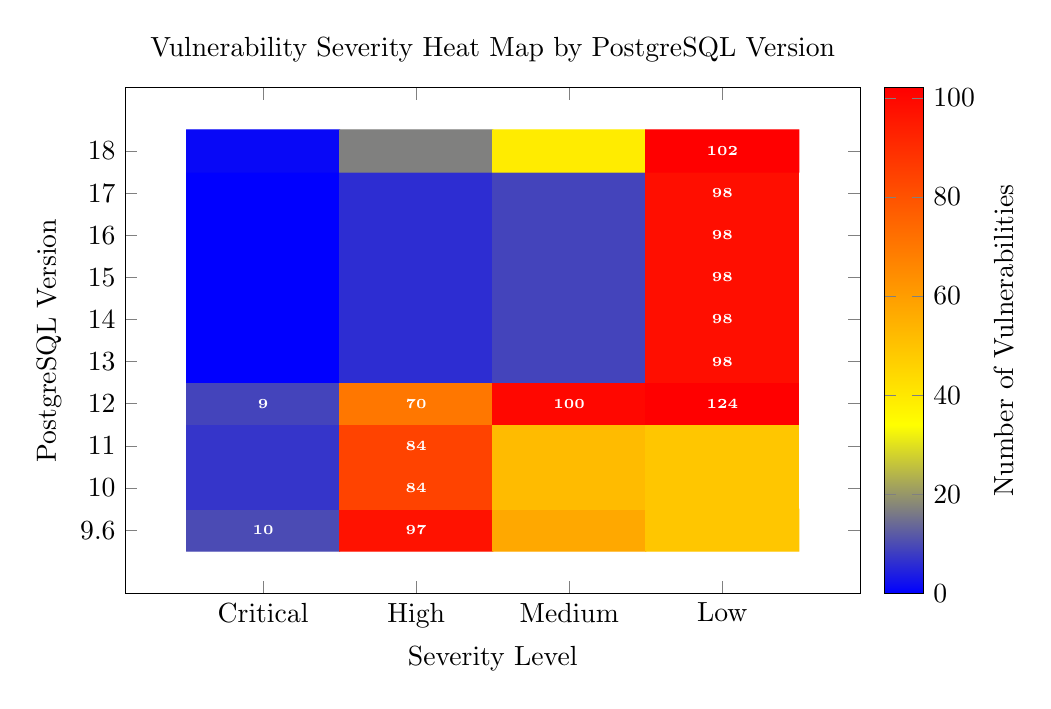
\begin{tikzpicture}
\begin{axis}[
    width=0.9\textwidth,
    height=8cm,
    title={Vulnerability Severity Heat Map by PostgreSQL Version},
    xlabel={Severity Level},
    ylabel={PostgreSQL Version},
    symbolic x coords={Critical, High, Medium, Low},
    symbolic y coords={9.6, 10, 11, 12, 13, 14, 15, 16, 17, 18},
    xtick=data,
    ytick=data,
    colormap/hot,
    colorbar,
    colorbar style={ylabel=Number of Vulnerabilities},
    point meta min=0,
    point meta max=102,
]

% Data points for heat map (version, severity, count)
\addplot[matrix plot*, mesh/cols=4, point meta=explicit] coordinates {
    (Critical,9.6)  [10]  (High,9.6)  [97]  (Medium,9.6)  [57]  (Low,9.6)  [49]
    (Critical,10)   [7]   (High,10)   [84]  (Medium,10)   [52]  (Low,10)   [49]
    (Critical,11)   [7]   (High,11)   [84]  (Medium,11)   [52]  (Low,11)   [49]
    (Critical,12)   [9]   (High,12)   [70]  (Medium,12)   [100] (Low,12)   [124]
    (Critical,13)   [0]   (High,13)   [6]   (Medium,13)   [9]   (Low,13)   [98]
    (Critical,14)   [0]   (High,14)   [6]   (Medium,14)   [9]   (Low,14)   [98]
    (Critical,15)   [0]   (High,15)   [6]   (Medium,15)   [9]   (Low,15)   [98]
    (Critical,16)   [0]   (High,16)   [6]   (Medium,16)   [9]   (Low,16)   [98]
    (Critical,17)   [0]   (High,17)   [6]   (Medium,17)   [9]   (Low,17)   [98]
    (Critical,18)   [1]   (High,18)   [17]  (Medium,18)   [39]  (Low,18)   [102]
};

% Add value labels with white text for better visibility on dark backgrounds
\node at (axis cs:Critical,9.6) [white] {\tiny\bf 10};
\node at (axis cs:High,9.6) [white] {\tiny\bf 97};
\node at (axis cs:High,10) [white] {\tiny\bf 84};
\node at (axis cs:High,11) [white] {\tiny\bf 84};
\node at (axis cs:Critical,12) [white] {\tiny\bf 9};
\node at (axis cs:High,12) [white] {\tiny\bf 70};
\node at (axis cs:Medium,12) [white] {\tiny\bf 100};
\node at (axis cs:Low,12) [white] {\tiny\bf 124};
\node at (axis cs:Low,13) [white] {\tiny\bf 98};
\node at (axis cs:Low,14) [white] {\tiny\bf 98};
\node at (axis cs:Low,15) [white] {\tiny\bf 98};
\node at (axis cs:Low,16) [white] {\tiny\bf 98};
\node at (axis cs:Low,17) [white] {\tiny\bf 98};
\node at (axis cs:Low,18) [white] {\tiny\bf 102};

\end{axis}
\end{tikzpicture}
\caption{Heat map visualization showing vulnerability counts by severity and version. Darker colors indicate higher vulnerability counts.}
\label{fig:heatmap}
\end{figure}


\subsection{Cost-Benefit Analysis: Upgrade vs. Risk}

\begin{table}[htbp]
\centering
\caption{Upgrade Effort vs. Security Risk Assessment}
\label{tab:cost-benefit}
\begin{tabular}{@{}lccp{6cm}@{}}
\toprule
\textbf{Migration Path} & \textbf{Effort} & \textbf{Risk Reduction} & \textbf{Notes} \\ \midrule
\rowcolor{lightgreen} 13 $\rightarrow$ 14 & Low & High & Single major version jump, similar features \\
\rowcolor{lightgreen} 12 $\rightarrow$ 14 & Medium & Very High & 2 major versions, eliminates 9 critical CVEs \\
\rowcolor{lightorange} 11 $\rightarrow$ 15 & Medium & Very High & 4 major versions, significant feature changes \\
\rowcolor{lightred} 10 $\rightarrow$ 16 & High & Critical & 6 major versions, requires thorough testing \\
\rowcolor{lightred} 9.6 $\rightarrow$ 17/18 & Very High & Critical & 8-9 major versions, extensive compatibility review needed \\
\bottomrule
\end{tabular}
\end{table}

\textbf{Recommendation Strategy:}
\begin{itemize}
    \item \textbf{Step 1:} Upgrade to the minimum supported version (14) immediately to escape EOL status
    \item \textbf{Step 2:} Plan migration to version 16 or 17 for long-term support (EOL 2028-2029)
    \item \textbf{Step 3:} Establish regular minor update process to stay current within major version
\end{itemize}


\subsection{Vulnerability Comparison: 18.0 vs 18.1 vs 18.2}
\label{subsec:patch-comparison}

To illustrate the importance of patch releases, we compare the vulnerabilities found in \texttt{postgres:18} versions.

\begin{table}[htbp]
\centering
\caption{Vulnerability Comparison: PostgreSQL 18.0 vs 18.1 vs 18.2}
\label{tab:trivy-compare}
\begin{tabular}{@{}lccccc@{}}
	\textbf{Docker Tag} & \textbf{Critical} & \textbf{High} & \textbf{Medium} & \textbf{Low} & \textbf{Total} \\ \midrule
\rowcolor{lightorange} \texttt{postgres:18.0} & 4 & 30 & 68 & 102 & 204 \\
\rowcolor{lightgreen} \texttt{postgres:18.1} & 1 & 17 & 39 & 102 & 159 \\
\rowcolor{lightgreen} \texttt{postgres:18.2} & 1 & 17 & 39 & 102 & 159 \\
\bottomrule
\end{tabular}
\end{table}

\begin{figure}[htbp]
\centering
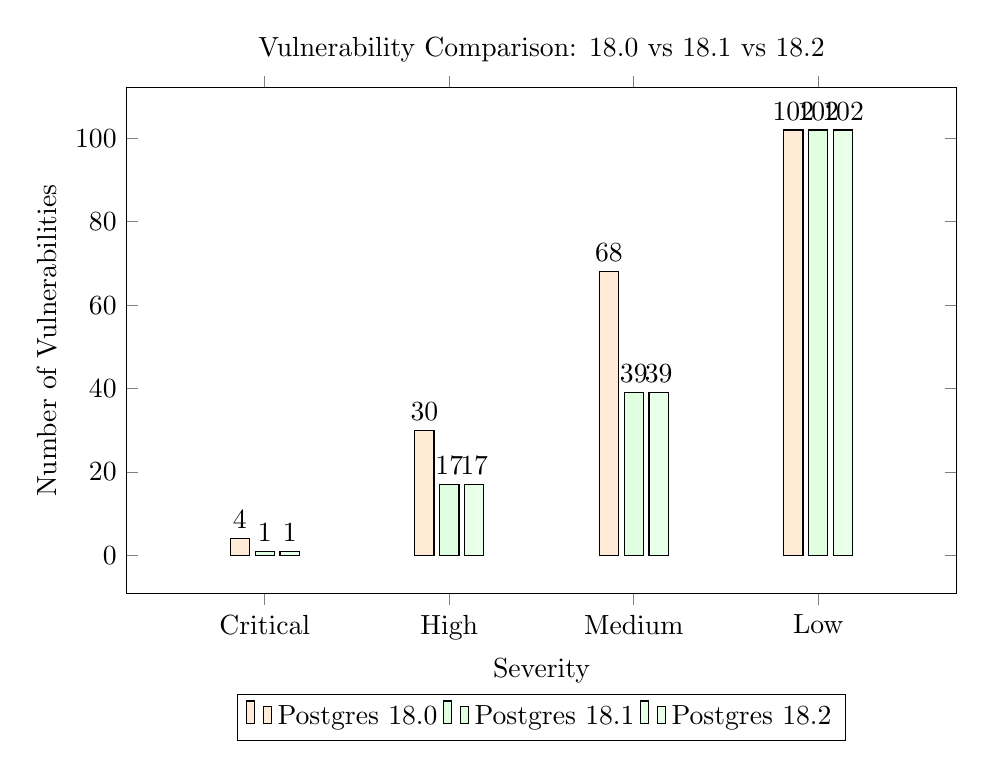
\begin{tikzpicture}
\begin{axis}[
    ybar=2pt,
    bar width=7pt,
    width=\textwidth,
    height=8cm,
    title={Vulnerability Comparison: 18.0 vs 18.1 vs 18.2},
    xlabel={Severity},
    ylabel={Number of Vulnerabilities},
    symbolic x coords={Critical, High, Medium, Low},
    xtick=data,
    nodes near coords,
    nodes near coords align={vertical},
    legend style={at={(0.5,-0.2)}, anchor=north, legend columns=3},
    enlarge x limits=0.25
]
\addplot[fill=lightorange!80] coordinates {(Critical,4) (High,30) (Medium,68) (Low,102)};
\addplot[fill=lightgreen!80] coordinates {(Critical,1) (High,17) (Medium,39) (Low,102)};
\addplot[fill=lightgreen!60] coordinates {(Critical,1) (High,17) (Medium,39) (Low,102)};
\legend{Postgres 18.0, Postgres 18.1, Postgres 18.2}
\end{axis}
\end{tikzpicture}
\caption{Comparison of vulnerabilities detected by \texttt{trivy} for PostgreSQL 18.0, 18.1 and 18.2. Grouped bars show clear reduction in critical and high severity issues.}
\label{fig:vuln-chart-18.0-18.1}
\end{figure}

The updates from 18.0 to 18.1 and then to 18.2 significantly reduced the number of critical, high, and medium vulnerabilities, demonstrating the effectiveness of minor releases in addressing security issues. For detailed changes, refer to the respective changelogs: \href{https://www.postgresql.org/docs/18/release-18.html}{18.0}, \href{https://www.postgresql.org/docs/18/release-18-1.html}{18.1}, and \href{https://www.postgresql.org/docs/18/release-18-2.html}{18.2}.

\section{Recommendations}

Based on the comprehensive security analysis presented in this report, the following actions are recommended:

\subsection{Immediate Actions (Critical Priority)}

\begin{itemize}
    \item \textbf{Migrate from EOL Versions:} If currently running PostgreSQL versions $\leq$13, plan immediate migration to version $\geq$14. These versions contain 2-10× more vulnerabilities.
    \item \textbf{Audit Current Deployments:} Use \texttt{geol check psql --version X} to verify your PostgreSQL version status in CI/CD pipelines.
    \item \textbf{Scan Docker Images:} Integrate \texttt{trivy image postgres:X --severity CRITICAL,HIGH} into deployment workflows.
\end{itemize}

\subsection{Long-Term Strategy}

\begin{itemize}
    \item \textbf{Target Version Selection:}
    \begin{itemize}
        \item Minimum: PostgreSQL 14 (EOL Nov 2026) - escape EOL status
        \item Recommended: PostgreSQL 16-17 (EOL 2028-2029) - optimal support window
        \item Latest: PostgreSQL 18 (EOL Nov 2030) - maximum future-proofing
    \end{itemize}
    \item \textbf{Patch Management:} Establish automated monitoring for minor releases - as shown in Section \ref{subsec:patch-comparison}, patches can reduce vulnerabilities by 22\% or more.
    \item \textbf{Docker Tag Strategy:} Use specific version tags (e.g., \texttt{postgres:17.7}) instead of major version tags to control updates.
\end{itemize}

\subsection{DevSecOps Integration}

\begin{itemize}
    \item Implement automated EOL checking in quality gates
    \item Set up vulnerability scanning as a deployment prerequisite
    \item Schedule quarterly reviews of PostgreSQL version lifecycle status
    \item Document upgrade paths and maintain rollback procedures
\end{itemize}

\section{Summary and conclusion}

The combined data analysis is clear. Figure \ref{fig:vuln-chart} strikingly illustrates this divergence:

\begin{itemize}
    \item \textbf{The danger of unsupported versions:} Versions that have reached their end of life (12, 11, 10, 9.6) accumulate a dangerous number of vulnerabilities, including several \textbf{critical} ones.
    \item \textbf{The security of supported versions:} In contrast, images of maintained versions (14 to 18) show no critical vulnerabilities and a low, consistent risk profile. Note that PostgreSQL 13 is now unsupported.
    \item \textbf{Recommendation:} The choice of PostgreSQL version must be for an actively supported version. The security risk of using an obsolete version is real and high.\\
\end{itemize}

Tools like \texttt{geol} and \texttt{trivy} are essential in a modern DevSecOps approach. This analysis of PostgreSQL perfectly illustrates how abandoning software support directly leads to a drastic increase in security flaws. Using up-to-date versions is not just a recommendation, but a necessity for the security of any infrastructure.

\section{Resources}

\begin{itemize}
    \item \href{https://dev.to/adriens/geol-the-cli-to-efficiently-manage-eols-like-a-boss-3hne}{geol, the cli to efficiently manage EOLs like a boss}
    \item \href{https://youtu.be/ZqiXogK2fSw}{geol - Gérer la fin de vie (notebookLM slideshow) v1.3.0 - "for dummies" edition}
    \item \href{https://youtu.be/yCZRgAiQt9s}{geol 1.3.0 unboxing - the check command}
    \item \href{https://youtu.be/vhFXWGqB_-g}{MVP Unboxing geol - a devops secops cli to manage EOLs and product lifecycle}
    \item \href{https://github.com/adriens/geol-showcase}{geol-showcase, A set of resources to showcase what could be achieved with geol, datascience, AI and devsecops tools}
    \item \href{https://www.postgresql.org/about/news/postgresql-181-177-1611-1515-1420-and-1323-released-3171/}{PostgreSQL 18.1, 17.7, 16.11, 15.15, 14.20, and 13.23 Released!}
    \item \href{https://endoflife.date/postgresql}{PostgreSQL EOL Data}
\end{itemize}

\end{document}
